\documentclass[10pt,showpacs,preprintnumbers,footinbib,amsmath,amssymb,aps,prl,twocolumn,groupedaddress,superscriptaddress,showkeys]{revtex4-1}
\usepackage{graphicx}
\usepackage{dcolumn}
\usepackage{bm}
\usepackage[colorlinks=true,urlcolor=blue,citecolor=blue]{hyperref}
\usepackage{color}
\usepackage{listings}

\newcommand{\deriv}[3][]{% \deriv[<order>]{<func>}{<var>}
	\ensuremath{ \frac{d^{#1} {#2}}{d {#3}^{#1}} } }


\begin{document}
\title{Project 1}
\author{Thomas Redpath and Dayah Chrisman}
\affiliation{Department of Physics, Michigan State University}
\begin{abstract}

We solve the Lippman-Schwinger equation in momentum space for proton-neutron scattering to obtain the $l=0$
phase shift $\delta _0$ as a function of lab energy. We calculate the Reaction matrix $R_l(k_0,k_0)$, of which the
diagonal elemets are related to the phase shift for the corresponding momentum $k_0$. We compare our results to the $\delta _0$
extracted from experiment (Nijmegen Group, PRC 48 792 (1993)).

We solve the Lippman-Schwinger equation for proton-neutron scattering to obtain the $l=0$
phase shift $\delta _0$ as a function of lab energy. We compare our results to the $\delta _0$
extracted from experiment (Nijmegen Group, PRC 48 792 (1993)).

\end{abstract}
\maketitle

\section{Introduction}




\section{Theory and algorithms}\label{sec:theory}

\subsection{Lippman-Schwinger Equation}

In order to calculate the phase shifts $\delta_l$, we need to solve the Schr{\"o}dinger equation
for the neutron-proton system with $E > 0$. This can be expressed as an integral equation for
the reaction matrix

\begin{equation}
\begin{split}
    R_l(k,k') &= V_l(k,k') + \\
  &\frac{2}{\pi}\hat{P}
                \int_0^{\infty}dqq^2V_l(k,q)\frac{1}{E-q^2/m}R_l(q,k'),
   \label{eq:ls1}
\end{split}
\end{equation}
where $E = k _0 ^2 / m$ is the total kinetic energy of the nucleons in the center-of-mass
system and the momentum-space representation of the potential $V(k',k)$ is used. We solve this
equation numerically on a discretized domain where we've set the mesh points and
weights using Gaussian Legendre quadrature. We map the points and weights from the interval of
the Legendre polynomials ($x \in [-1,1]$) to our desired interval $r \in [0,\infty)$ using the
following mapping

\begin{align*}
          k_i&=const\times tan\left\{\frac{\pi}{4}(1+x_i)\right\} \\
          \omega_i&= const\frac{\pi}{4}\frac{w_i}{cos^2\left(\frac{\pi}{4}(1+x_i)\right)}.
\end{align*}

In order to ensure convergence, we performed calculations of the phase shifts vs. energy and showed that the curve converges to the analytic value for the infinite spherical well as more and more mesh points are added. This convergence can be seen in Figure 1. \\ \\

We summarize the prescription for solving eq.~\ref{eq:ls1} numerically from
\citet{lectureNotes}. First, we employ Cauchy's principle-value prescription
to re-write eq.~\ref{eq:ls1} in the form

\begin{equation}
\begin{split}
    R(k,k') &= V(k,k') + \\
   & \frac{2}{\pi}
                \int_0^{\infty}dq
                \frac{q^2V(k,q)R(q,k')-k_0^2V(k,k_0)R(k_0,k')  }
                     {(k_0^2-q^2)/m},
   \label{eq:ls2}
\end{split}
\end{equation}
which is represented on the discretized mesh as

\begin{equation}
\begin{split}
R(k,k') &= V(k,k') +\frac{2}{\pi}\sum_{j=1}^N\frac{\omega_jk_j^2V(k,k_j)R(k_j,k')}{(k_0^2-k_j^2)/m}- \\
  & \frac{2}{\pi}k_0^2V(k,k_0)R(k_0,k')\sum_{n=1}^N\frac{\omega_n}{(k_0^2-k_n^2)/m},
\end{split}
\label{eq:ls3}
\end{equation}
where there are $N$ mesh points from the Gaussian quadrature mapping
and one point that is the chosen ``observable'' point corresponding to the
relative momentum for which we want to calculate the phase shift. Total
there are $(N+1)$ mesh points.

Next, we organize eq.~\ref{eq:ls3} as a matrix equation by defining a
matrix $A$

\begin{equation*}
	A_{i,j} = \delta _{i,j} - V(k_i,k_j)u_j
\end{equation*}
where

\begin{equation}
     u_j=\frac{2}{\pi}
         \frac{\omega_jk_j^2}{(k_0^2-k_j^2)/m}\hspace{1cm}
         j=1,N
\label{eq:uj}
\end{equation}
and

\begin{equation}
     u_{N+1}=-\frac{2}{\pi}
          \sum_{j=1}^N\frac{k_0^2\omega_j}{(k_0^2-k_j^2)/m}.
\label{eq:u0}
\end{equation}

We can now solve for the $R$ matrix by inverting the matrix $A$ and multiplying $V$
by $A^{-1}$. Finally, the $R(N+1,N+1)$ element is related to the phase
shift for $k_0$ by

\begin{equation}
	R(k_0,k_0)=-\frac{tan\delta}{mk_0}
	\label{eq:PhaseShift}
\end{equation}
Using this prescription and some model for the interaction (see next
subsection), we can calculate $\delta$ for scattering at some incident energy.
We describe the \texttt{C++} code used to make these calculations in
the Methods section.


\subsection{Potential Model}

We currently have coded two potentials that can be used in the phase shift
calculation. The first is a finite square well (eq.~\ref{eq:FSpot}) used to
benchmark the program against the analytical result. The second is a
parameterized $^1S_0$ neutron-proton interaction (eq.~\ref{eq:NPpot}).

\begin{equation}
	V = -V_0 \Theta(a - r)
	\label{eq:FSpot}
\end{equation}

\begin{equation}
	V(r)=V_a \frac{e^{-ax}}{x}+V_b \frac{e^{-bx}}{x}+V_c \frac{e^{-cx}}{x},
	\label{eq:NPpot}
\end{equation}
with $x=\mu r$, $\mu=0.7$ fm$^{-1}$ (the inverse of the pion mass),
$V_a=-10.463$ MeV and $a=1$, $V_b=-1650.6$ MeV and $b=4$ and
$V_c=6484.3$ MeV and $c=7$.

For both potentials, we find the momentum-space representations using
the Fourier-Bessel transform, we specialize to the case $l=0$ since we're
only aiming to calculate the $\delta_0$. For the finite well potential we
have

\begin{align*}
	V_l(k,k')&= \int j_l(kr)V(r)j_l(k'r)r^2dr\\
	&= V_0 \int_0^a \frac{\sin(kr) \sin(k'r) r^2}{k k' r^2} dr\\
	&= \frac{V_0}{k k'} \int_0^a \sin(kr) \sin(k'r) dr\\
	&= \frac{V_0}{k k'} \frac{k' \sin(ka) \cos(k'a) - k \cos(ka) \sin(k'a)}{k^2 - k'^2}
\end{align*}
This results in 

\begin{equation}
	V(k,k') = \frac{k_j \sin()\cos() + \cos()\sin()}{}
\end{equation}


\subsection{Reaction Matrix}


%\subsection*{The General Algorithm}

%\[
%\begin{bmatrix}
%	d_1 & a_1 & 0 & \dots & \dots & 0 \\
%	c_1 & d_2 & a_2 & 0 & \dots & 0 \\
%	0 & c_2 & d_3 & a_3 & 0 & \dots \\
%	\vdots & & \ddots & \ddots & \ddots & \vdots \\
%	\vdots & & & c_{n-2} & \ddots & a_{n-1}\\
%	0 & & & & c_{n-1} & d_n \\
%\end{bmatrix}
%~
%\begin{bmatrix}
%	u_1\\
%	u_2\\
%	u_3\\
%	u_4\\
%	\vdots\\
%	u_n\\
%\end{bmatrix}
%~
%=
%~
%\begin{bmatrix}
%	f_1\\
%	f_2\\
%	f_3\\
%	f_4\\
%	\vdots\\
%	f_n\\
%\end{bmatrix}
%\]

\section{Methods}

We implemented our numerical solution to the Lippman-Schwinger equation as a \texttt{C++} class.
This class consists of three two-dimensional data structures to hold the $V$, $A$ and $R$ matrices,
two one-dimensional data structures to hold the weights and momentum mesh points that define the
integration domain and several ancillary variables that specify the nucleon mass and other book-keeping
parameters. Application of the algorithms sketched in the previous section is carried out in a series of
member functions that (a) set up the mesh points and weights (b) set up the potential matrix (c) set
up the $A$ matrix (d) invert $A$ to get $R$ then extract $\delta _0$. In principle,
different functions may be used to set up different potentials; we coded one for the model NN interaction
given above and one for a finite spherical well to check that we recover the analytic result.
This class is defined in the source
file \texttt{NucleonScattering.cpp} and \texttt{NucleonScattering.hh}. An instance of the class is
created and the correct sequence of methods is called in the \texttt{main} function defined in
\texttt{main.cpp}.


%% -------------------------- CODE LISTING -------------------------- %%

%% 
 \definecolor{mygreen}{rgb}{0,0.6,0}
 \definecolor{mygray}{rgb}{0.5,0.5,0.5}
 \definecolor{mymauve}{rgb}{0.58,0,0.82}

 \lstset{ %
   backgroundcolor=\color{white},   % choose the background color; you must add \usepackage{color} or \usepackage{xcolor}
   basicstyle=\footnotesize,        % the size of the fonts that are used for the code
   breakatwhitespace=false,         % sets if automatic breaks should only happen at whitespace
   breaklines=true,                 % sets automatic line breaking
   captionpos=b,                    % sets the caption-position to bottom
   commentstyle=\color{mygreen},    % comment style
   deletekeywords={...},            % if you want to delete keywords from the given language
   escapeinside={\%*}{*)},          % if you want to add LaTeX within your code
   extendedchars=true,              % lets you use non-ASCII characters; for 8-bits encodings only, does not work with UTF-8
   frame=single,	                   % adds a frame around the code
   keepspaces=true,                 % keeps spaces in text, useful for keeping indentation of code (possibly needs columns=flexible)
   keywordstyle=\color{blue},       % keyword style
   language=C++,                 % the language of the code
   otherkeywords={*,...},           % if you want to add more keywords to the set
   numbers=left,                    % where to put the line-numbers; possible values are (none, left, right)
   numbersep=5pt,                   % how far the line-numbers are from the code
   numberstyle=\tiny\color{mygray}, % the style that is used for the line-numbers
   rulecolor=\color{black},         % if not set, the frame-color may be changed on line-breaks within not-black text (e.g. comments (green here))
   showspaces=false,                % show spaces everywhere adding particular underscores; it overrides 'showstringspaces'
   showstringspaces=false,          % underline spaces within strings only
   showtabs=false,                  % show tabs within strings adding particular underscores
   stepnumber=2,                    % the step between two line-numbers. If it's 1, each line will be numbered
   stringstyle=\color{mymauve},     % string literal style
   tabsize=2,	                   % sets default tabsize to 2 spaces
   title=\lstname                   % show the filename of files included with \lstinputlisting; also try caption instead of title
 }

 %\lstinputlisting[linerange={78-90}]{../src/proj1.cc}


\section{Results and discussion}

As a check, we calculate
$\delta _0$ from the analytic formula for the simple finite square well case phase shifts

\begin{equation}
	\delta _0(E) = \arctan \left [ \sqrt{\frac{E}{E+V_0}} \tan \left ( R \sqrt{2 \mu (E + V_0)}
 \right ) \right ] - R \sqrt{2 \mu E}
	\label{eq:deltaAnalytic}
\end{equation}
where
\begin{equation*}
	E = \frac{k^2}{2 \mu}
\end{equation*}


\subsection{Variable Phase Approach}
The variable phase approach relies on numerical methods to solve a differential equation.
Without including tensor forces,
it is limited to local potentials ($<r'|V|r>=^3\delta(r-r')V(r)$). However, the VPA is simple to use,
and information about the potential is relatively easy to extract. For example, here we show
that the presence of bound states (and the number of them) for a certain potential depth can
be determined from VPA calculations, and short-range repulsive components of the potential can
be inferred based on phase shift calculations at various energies.

The Variable Phase Approach relies on an incoming momentum and the potential depth.
Then, we inegrate over $r$ out to a sufficiently large radius ($R_max$) which is much larger
than the range of the potential. 

\begin{figure}
\centering
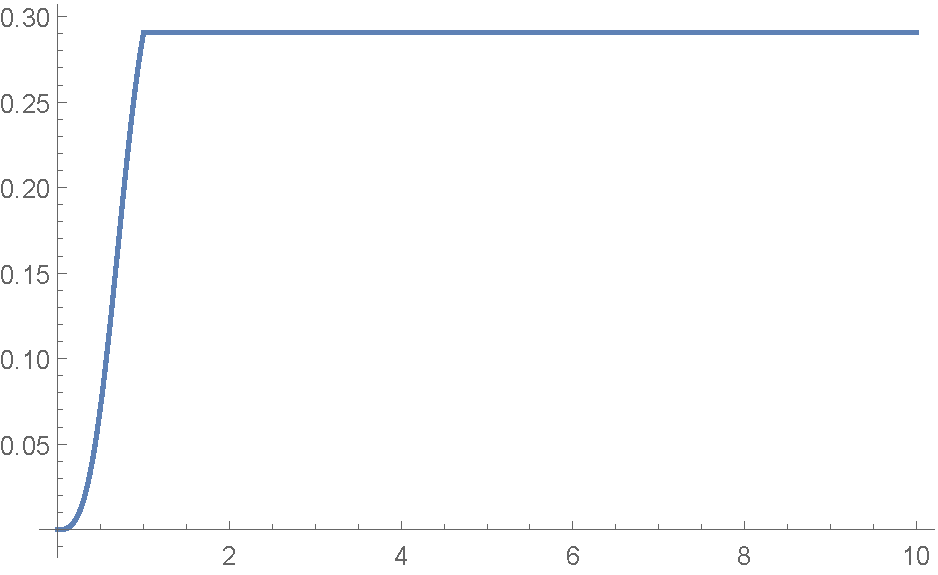
\includegraphics[width=0.45\textwidth]{figures/VPA_plot.pdf}
\caption{Phase shift as a function of radius.}
\label{fig:VPA}
\end{figure}

In Figure~\ref{fig:VPA}, we note that the phase shift becomes constant after a radius of 1;
this is the radius of the square well potential. Because of the discontinuity in the potential at the
edge of the square well, there is no ambiguity about how large we need to make our integration
radius: obviously, as soon as we are looking beyond the radius of potential, the phase shift will
stay a constant value. This tells us that any radius larger than 1 will give us a constant phase shift.

We then examined the plots of $k\cot(\delta)$ and $\delta$ to test Levinson's Theorem,
which states that the number of bound states can be calculated by looking at $\delta(E=0)$
and the limit of $\delta$ as $E$ approaches $\inf$

\begin{equation*}
	\phi_l(0)-\phi_l(\inf)=n\pi
\end{equation*}

where $n$ is the number of bound states the potential can hold. For a well depth $V_c=1.0$,
$\phi_l(0)=0$,  $\phi_l(\inf)=0$. This means that this well depth cannot produce a bound state
with $l=0$. For a well depth $V_c=2.0$, however,  $\phi_l(0)=3.14$,  $\phi_l(\inf)=0$, meaning
this deep of a square  well can hold 1 $l=0$ bound state.

We add now a short-range repulsive potential and calculate the phase shifts using the VPA.The
sign of a phase shift can characterize a potential as attractive ($\delta_0>0$) or repulsive
($\delta_0<0$). Adding a repulsive term should begin to make a difference at higher
energies/momenta, where the approaching particles can get close enough to ``see'' the effect of
this core. At these higher energies, we should see the phase shift turn negative, indicating the
repulsive character of the potential. At $V_c=0$ (no repulsive part of the potential - attractive
only), and $\Phi_l(\infty)=0$ This indicates, as we have specified, a purely attractive potential.
Around $V_c~18$, we can see the phase shift turning over at around $k=10$. As we increase
the height of the repulsive potential, the phase shifts start to become negative at lower and
lower energies, until at $V_c=100$ the phase shift turns negative at only $k=6$. 

Because the nuclear force is repulsive at short distances ($V \rightarrow \infty, r \rightarrow 0$),
we can use calculated phase shifts from experimental cross sections and estimate the range
of the repulsive part of the nuclear force (Rc). The radius at which the phase shift changes is
almost constant once $V_c$ gets larger, suggesting convergence to a single value, from which
$R_c$ can then be extracted. 



%\begin{table}
%\centering
%	\begin{tabular}{ c | c c c }
%	 & \multicolumn{3}{c}{Time [$\mu$s]}\\
%	$n$ & General & Specialized & LU Decomp\\
%\hline
%	$10^{1}$ & 2       & 2       & 10 \\
%	$10^{2}$ & 7       & 5       & 3500 \\
%	$10^{3}$ & 62      & 50      & 1700000\\
%	$10^{4}$ & 600     & 555     & \\
%	$10^{5}$ & 6100    & 5100    & \\
%	$10^{6}$ & 32500   & 28300   & \\
%	$10^{7}$ & 244000  & 205000  & \\
%\hline
%	\end{tabular}
%	\caption{Summary of execution times for the algorithms used.
%	We note that the execution time can vary from run to run due
%	to variations in CPU load. The execution time also varies
%	from platform to platform.}
%	\label{tab:speedresults}
%\end{table}


%\begin{figure*}
%\centering
%	\includegraphics{figures/sols.pdf}
%	\caption{A comparison of the results from the numerical solution
%	(with various choices for the number of grid points) to the exact
%	result. The blue curve plots the numerical result with 10 grid
%	points, the green curve uses 100 grid points and the red curve
%	uses 1000 grid points. The black curve plots the exact result.
%	Good agreement with the exact result is obtained once 100 grid
%	points are used.}
%	\label{fig:compexact}
%\end{figure*}



\section{Conclusions}

%\begin{thebibliography}{99}
%\bibitem{miller2006} G.~A.~Miller, A.~K.~Opper, and E.~J.~Stephenson, Annu.~Rev.~Nucl.~Sci.~{\bf 56}, 253 (2006).
%\bibitem{Morten} M. Hjorth-Jensen, Computational Physics Lecture Notes Fall 2015, August 2015.
%\bibitem{Mslides} M. Hjorth-Jensen, Computational Physics Notes, compphysics.github.io
%\bibitem{Golub1996} G. Golub, C. Van Loan, \textit{Matrix Computations} (John Hopkins University Press, 1996)
%\end{thebibliography}

\bibliographystyle{plainnat}
\bibliography{refs}

\end{document}
